
\section{Venue}

At this point the most promising option that we have is the Duale Hochschule
Baden-Württemberg (DHBW). We are however still in investigating other options
at this point.

\subsection{DHBW}

\begin{tikzpicture}
  \begin{scope}[on background layer]
    \node[inner sep=0,outer sep=0] (main) {%
      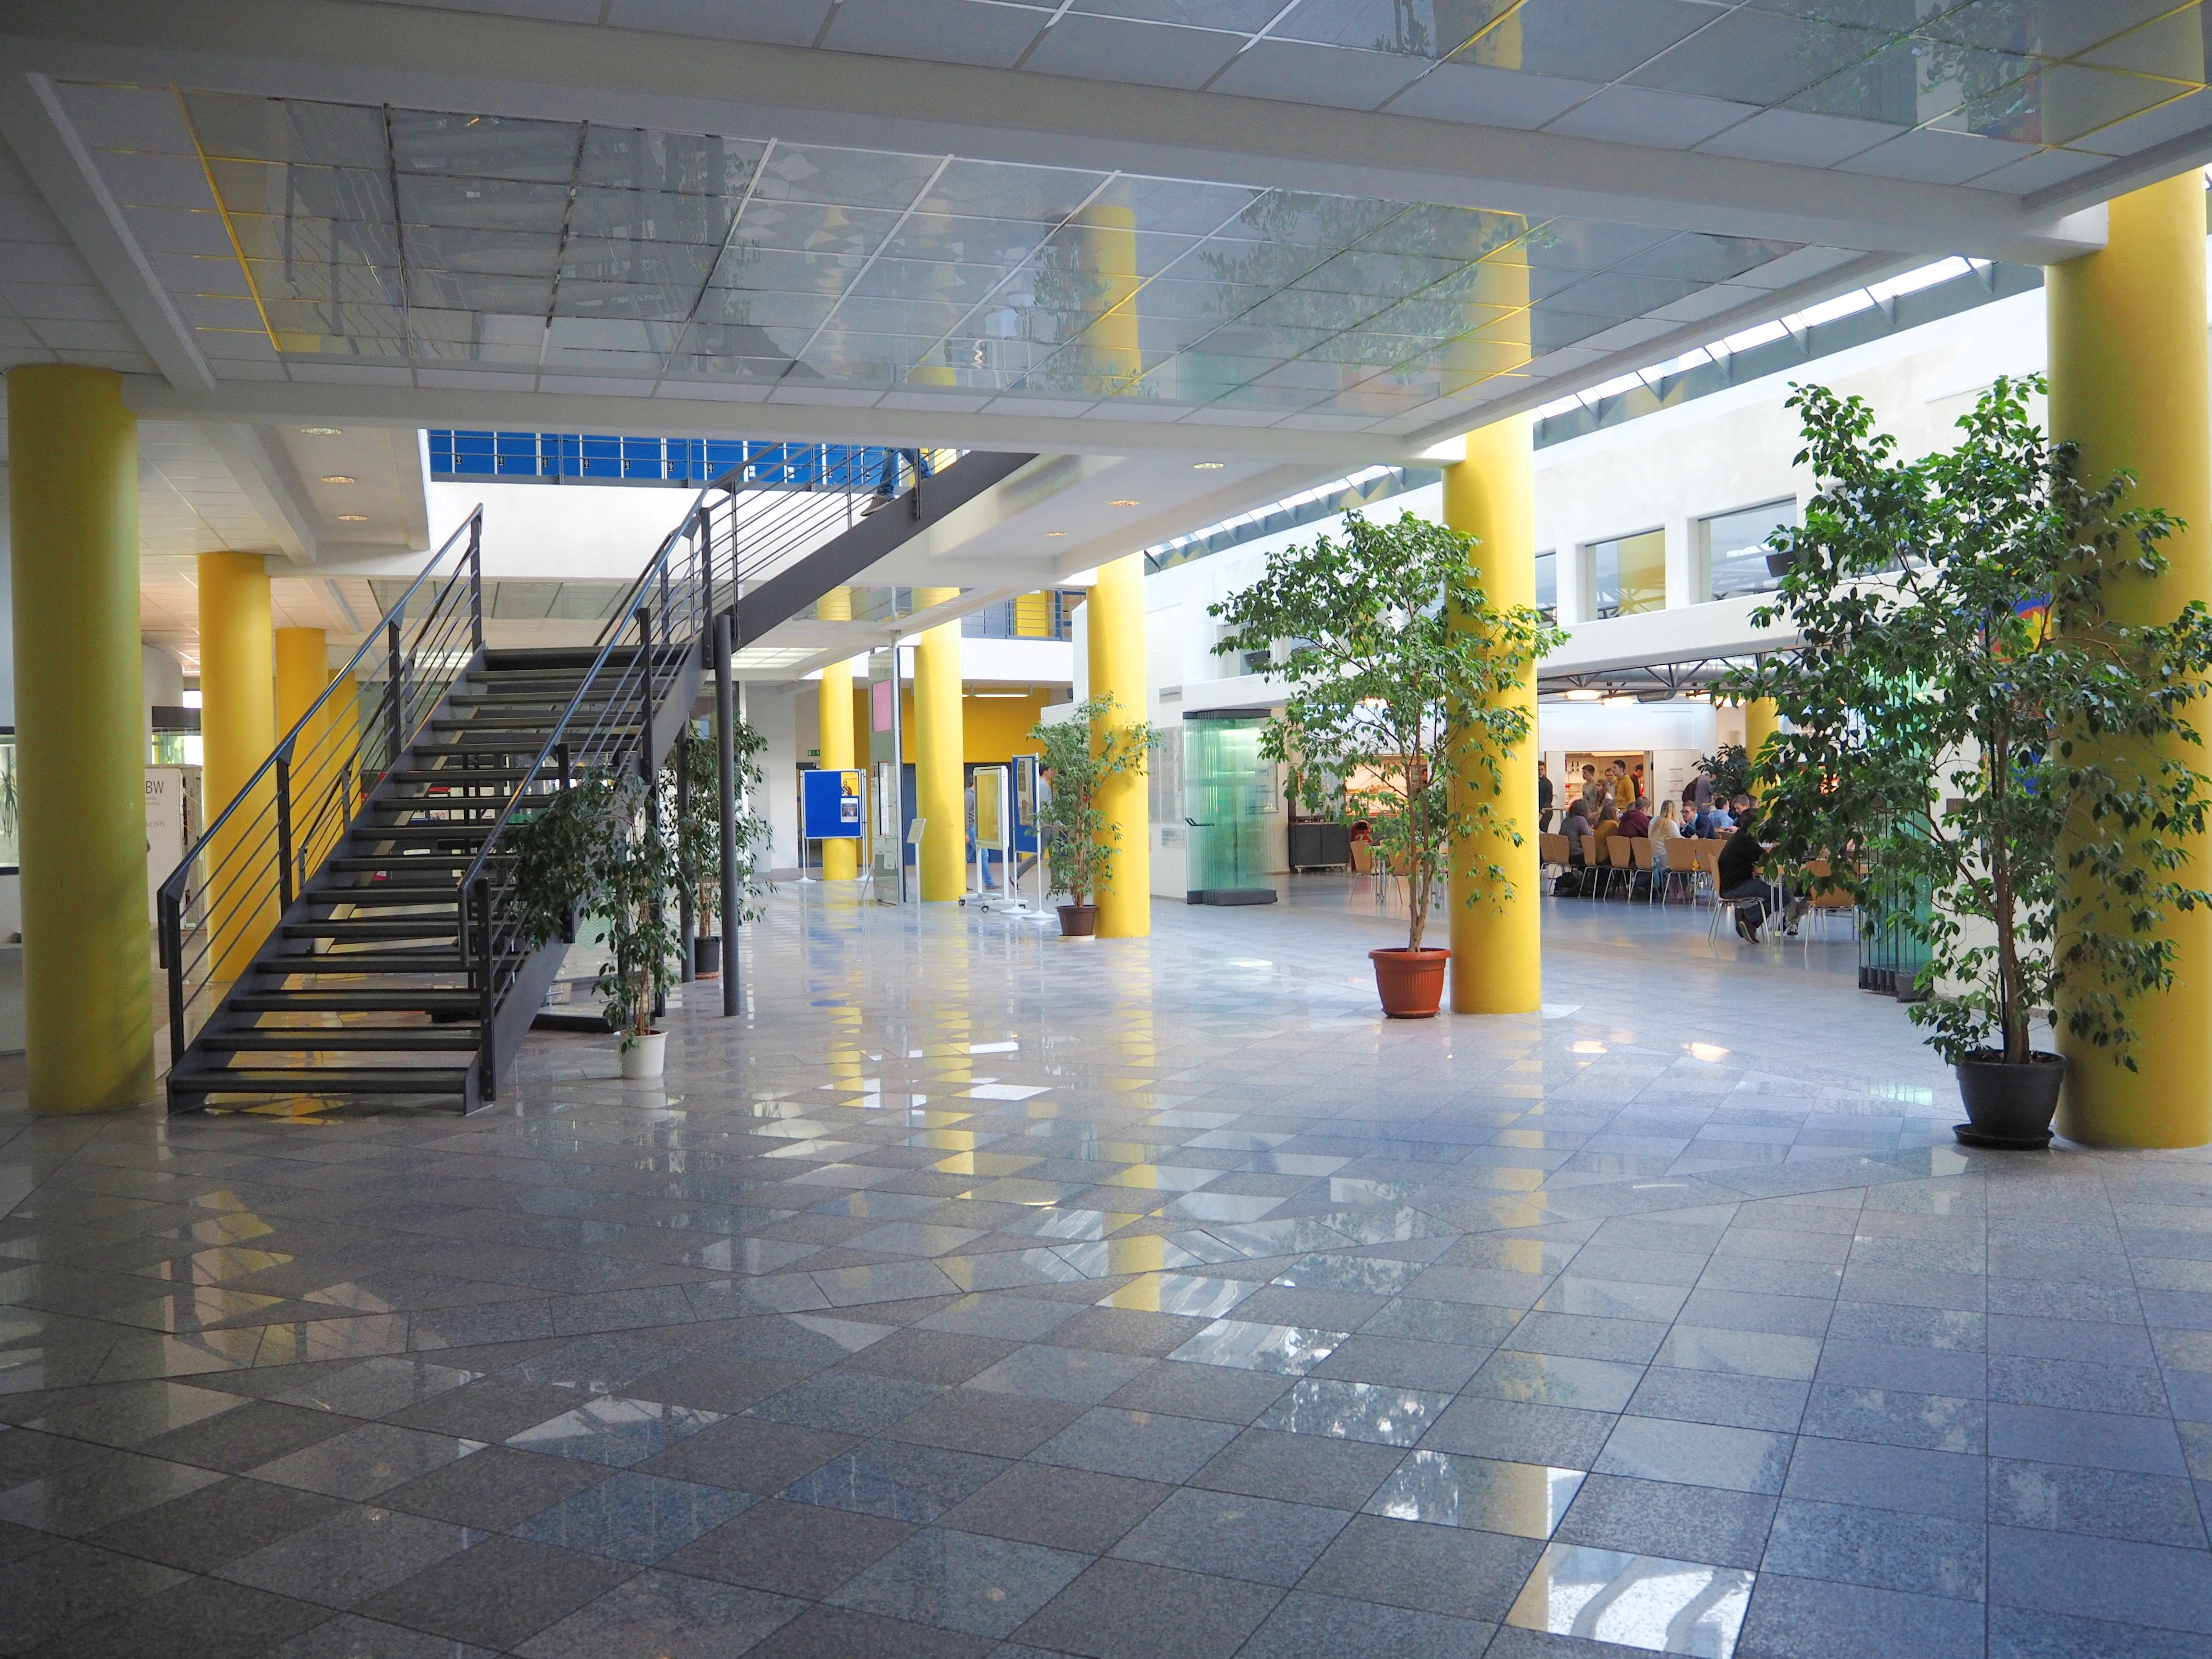
\includegraphics[width=0.5\linewidth]{images/venues/dhbw/P9280379}%
    };
    \node[inner sep=0,outer sep=0,anchor=north west] (sub-1) at (main.north east) {%
      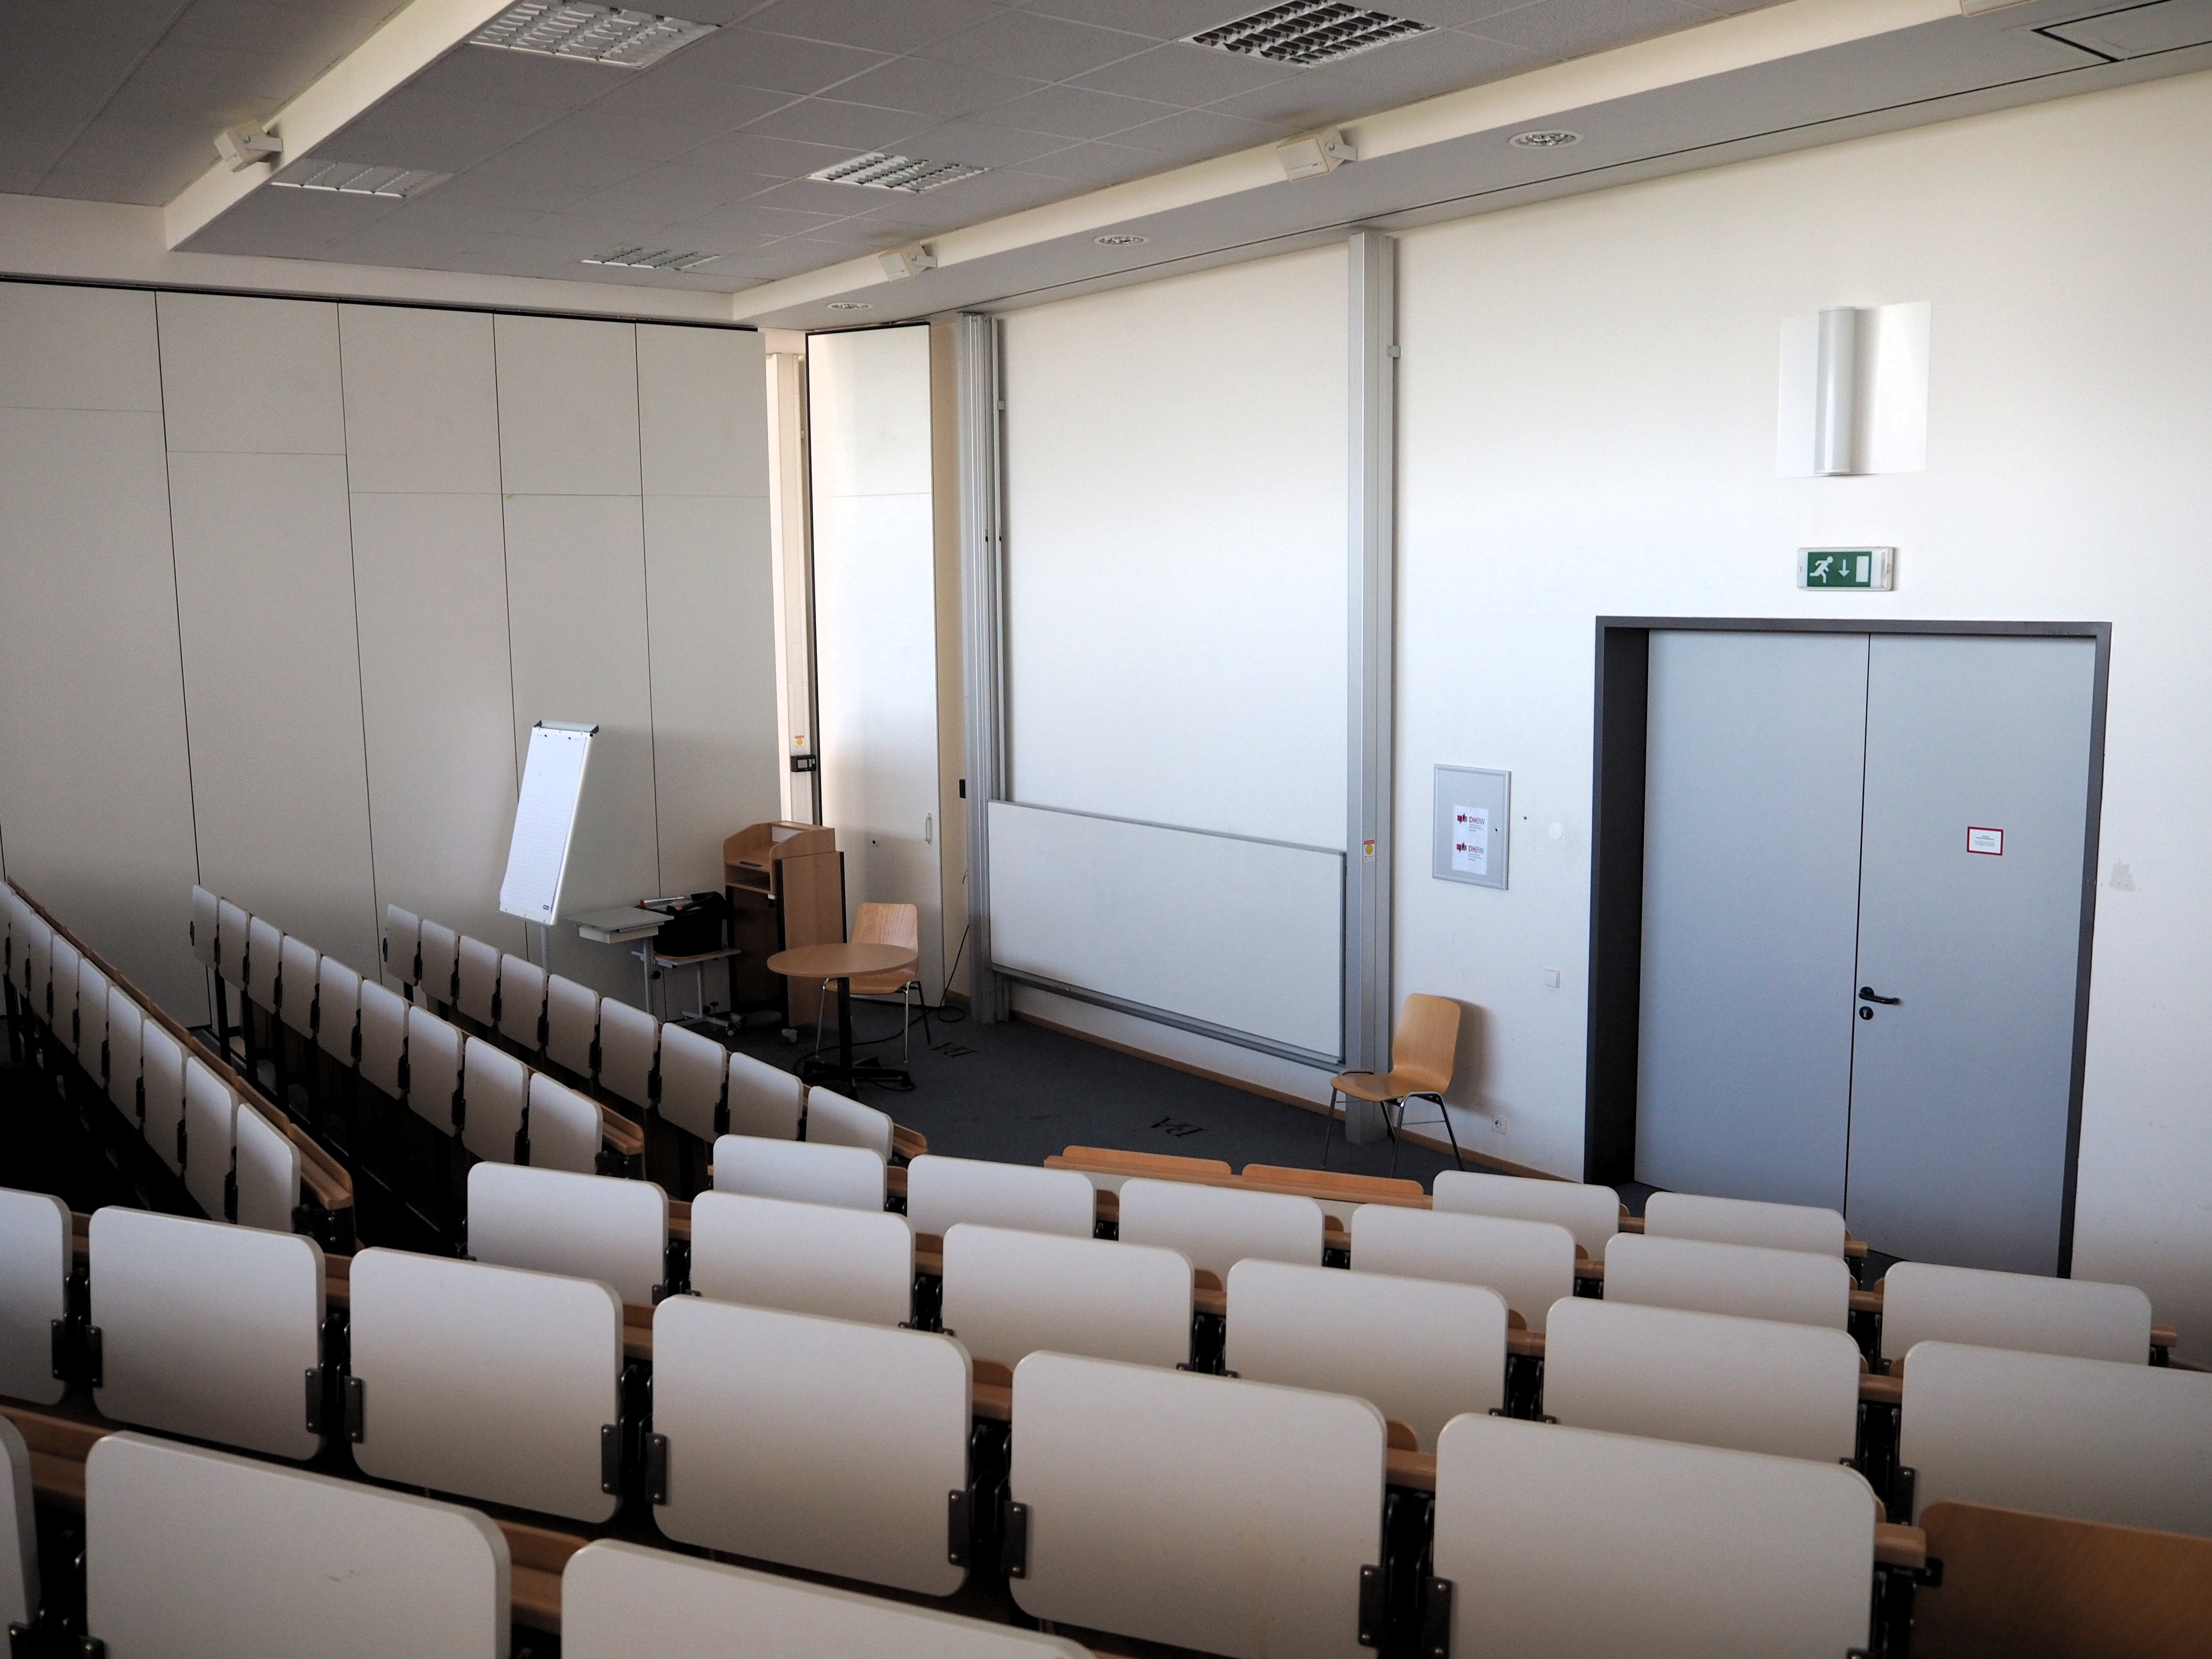
\includegraphics[width=0.25\linewidth]{images/venues/dhbw/P9280376}%
    };
    \node[inner sep=0,outer sep=0,anchor=north west] (sub-2) at (sub-1.south west) {%
      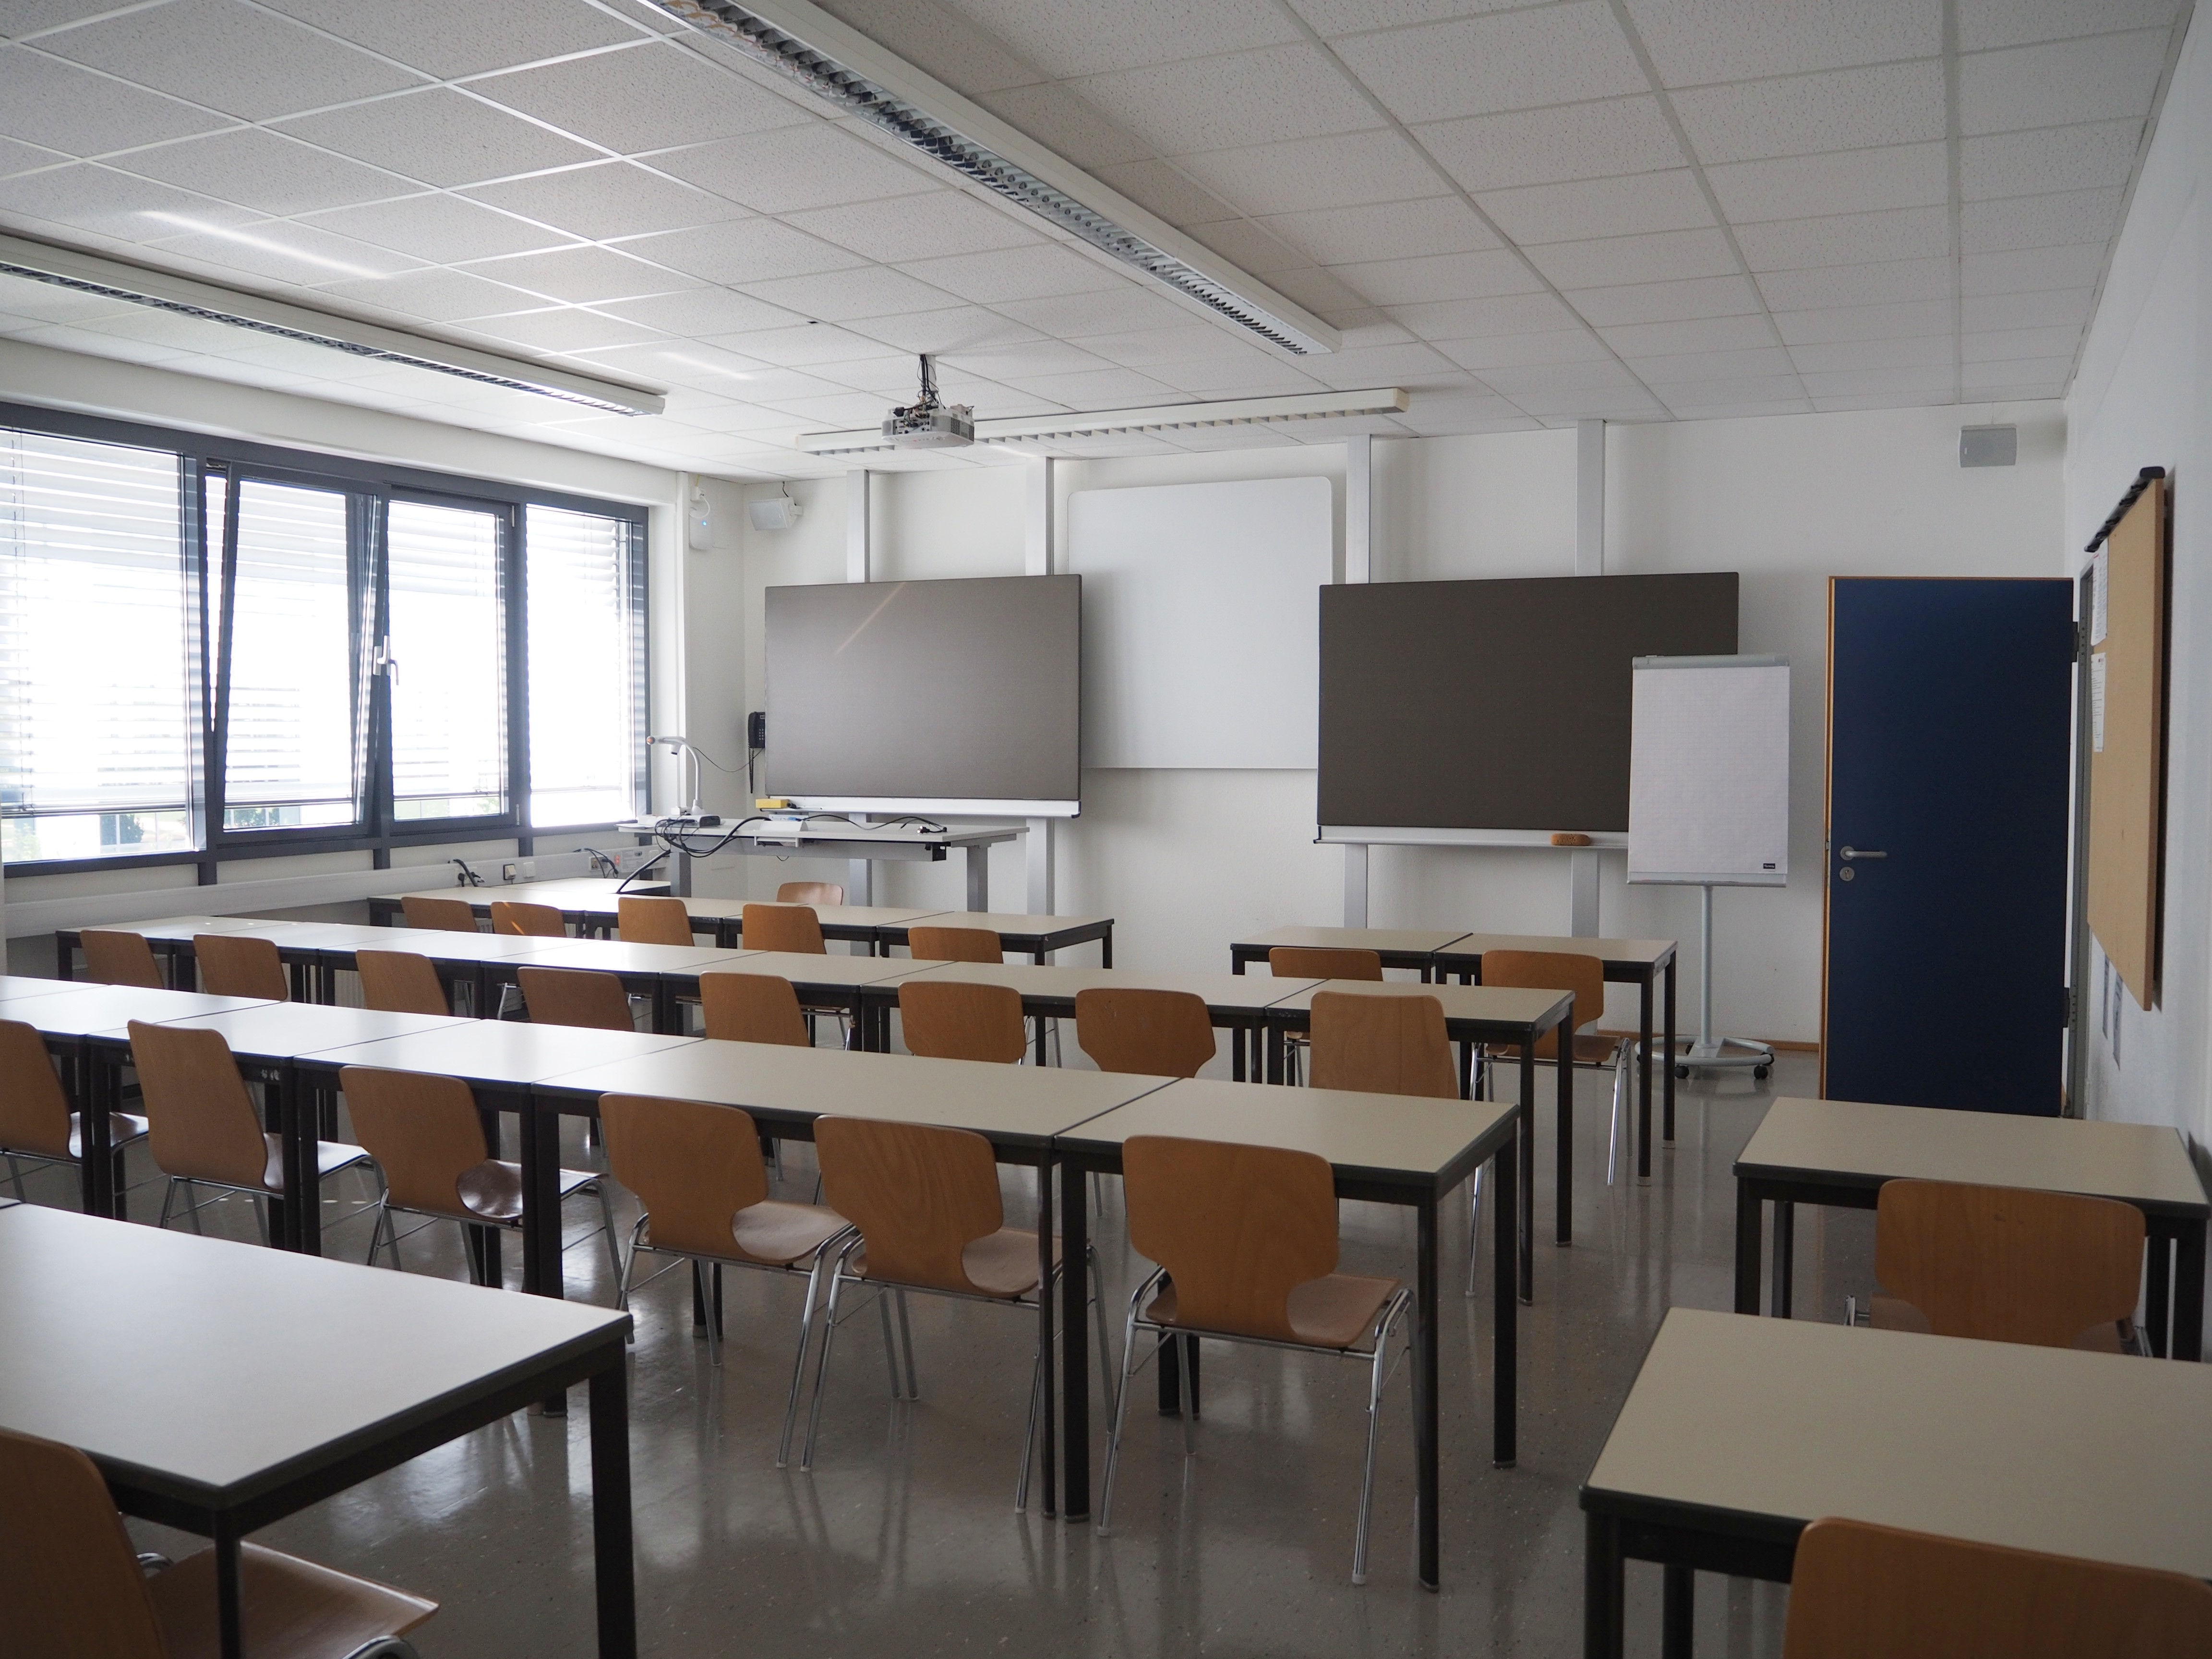
\includegraphics[width=0.25\linewidth]{images/venues/dhbw/P9280388}%
    };
    \node[inner sep=0,outer sep=0,anchor=north east] (sub-3) at (main.north west) {%
      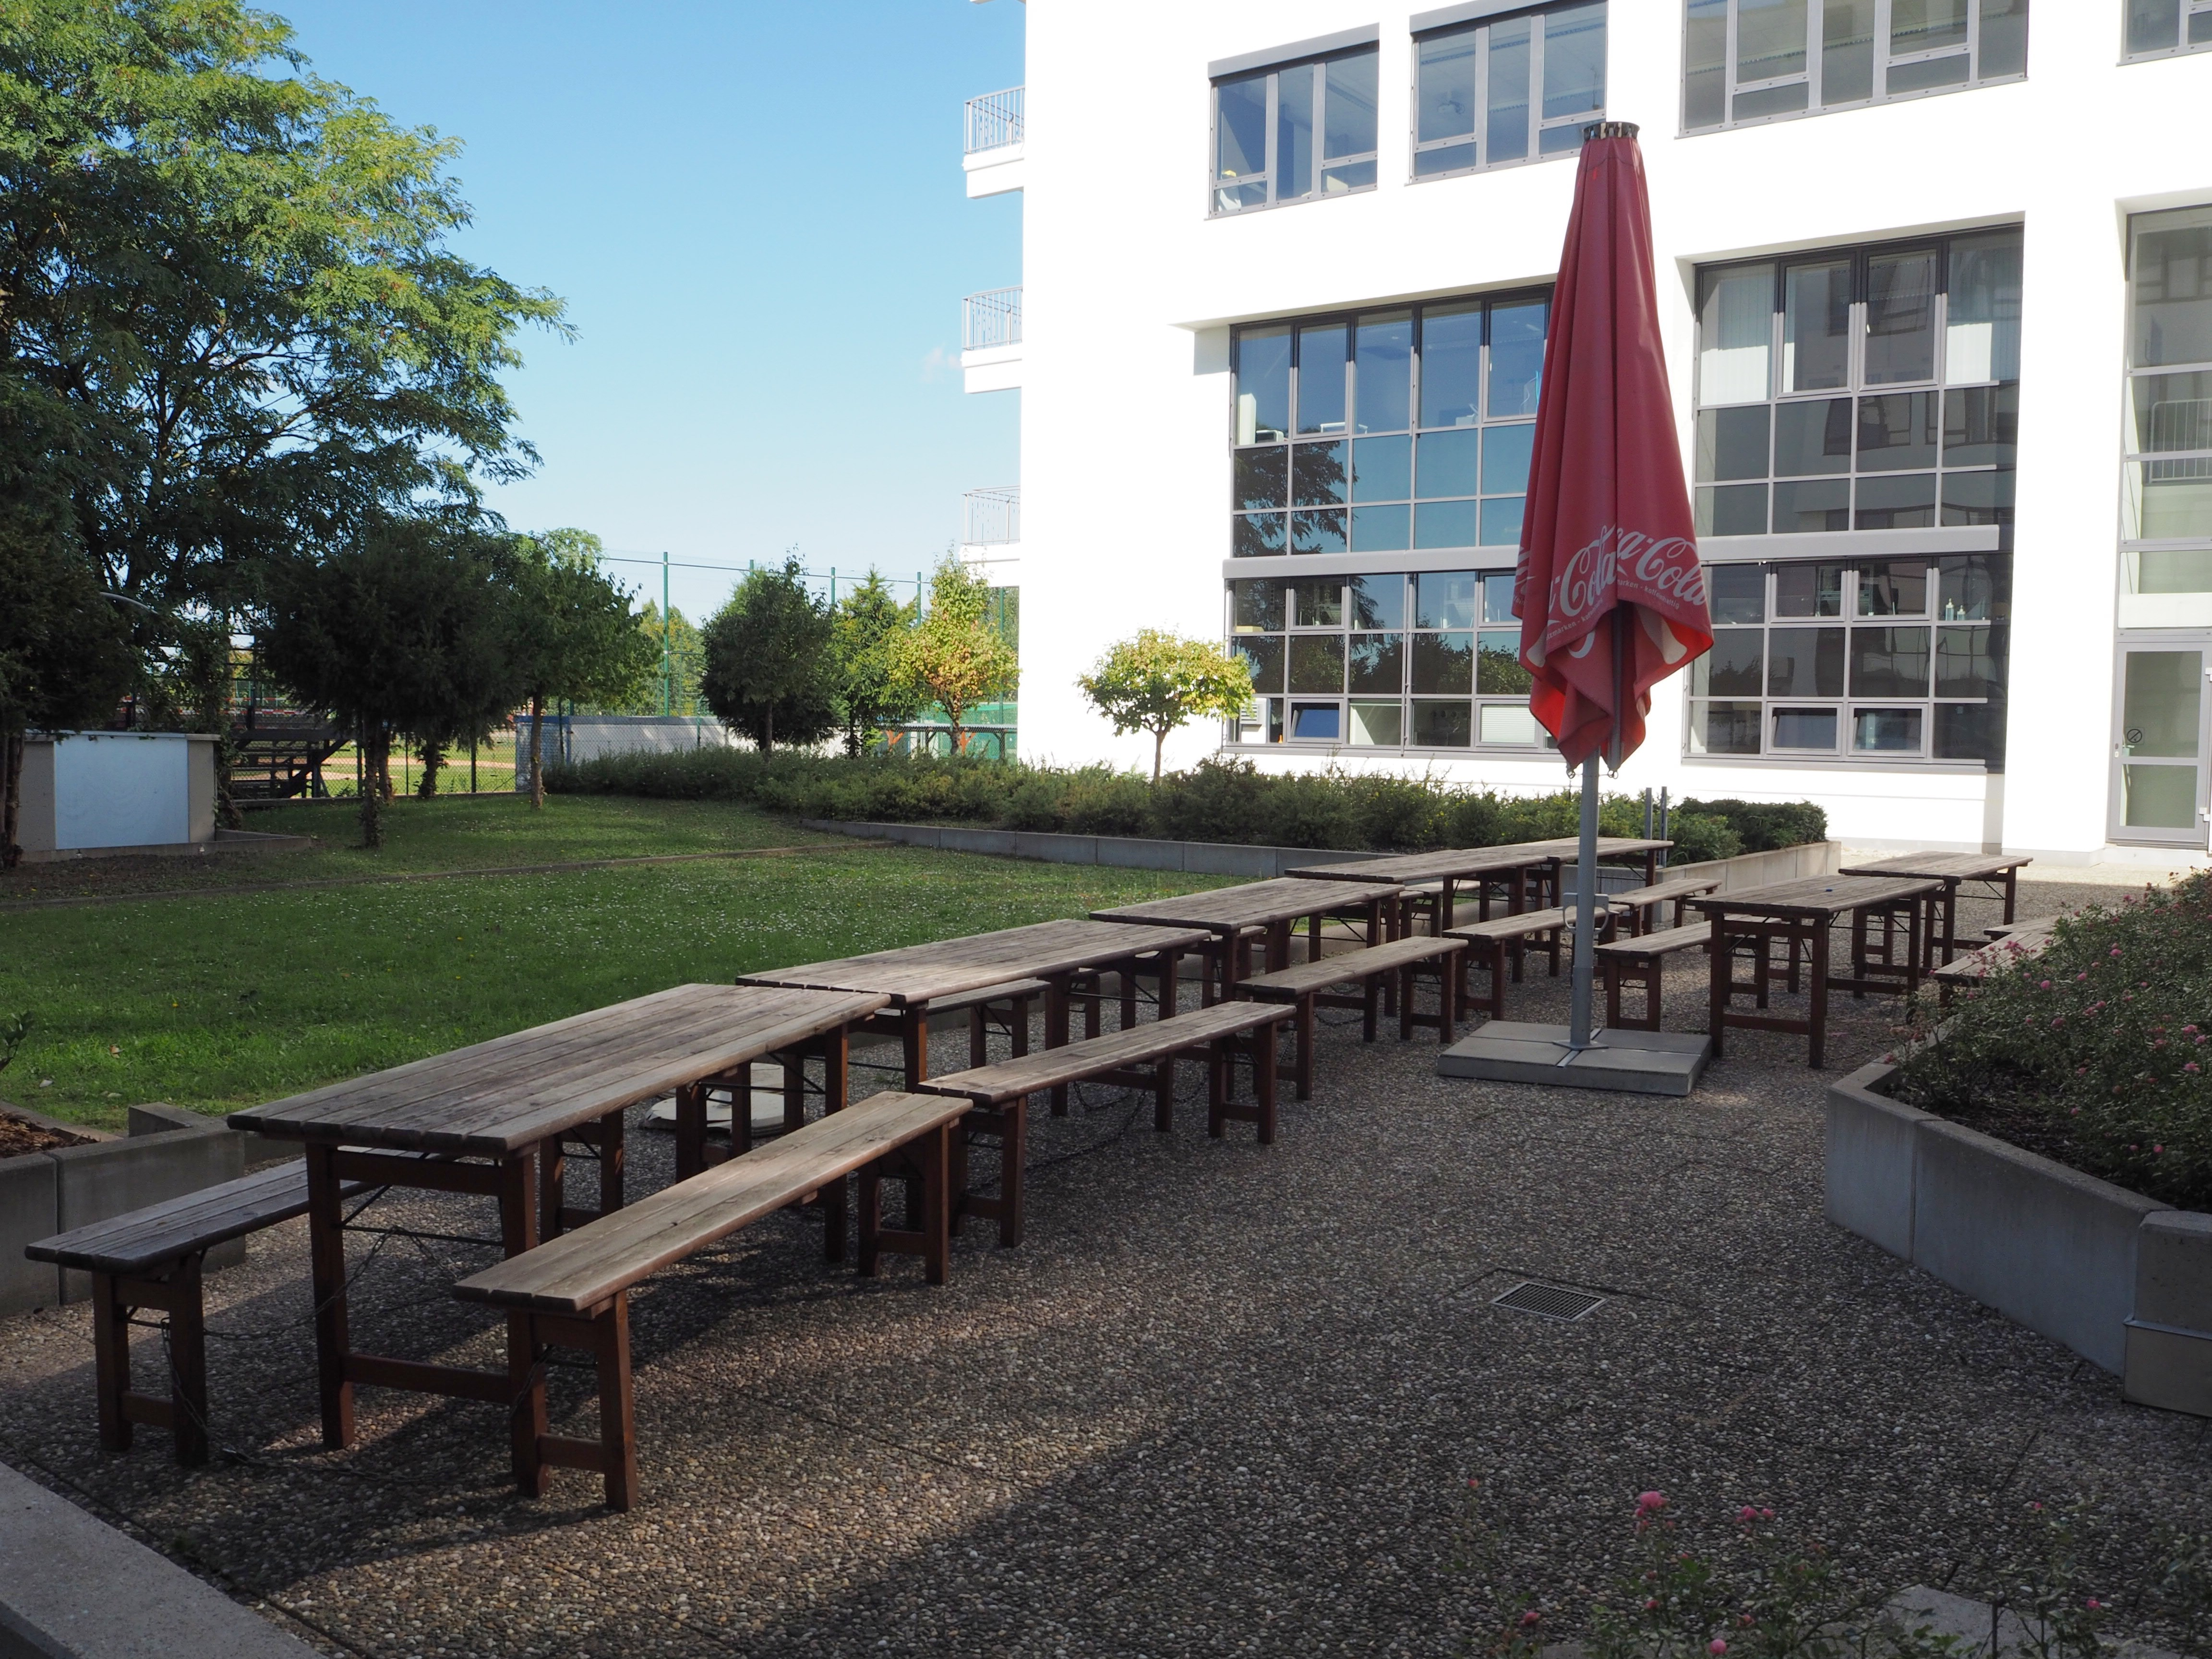
\includegraphics[width=0.25\linewidth]{images/venues/dhbw/P9280383}%
    };
    \node[inner sep=0,outer sep=0,anchor=north west] (sub-4) at (sub-3.south west) {%
      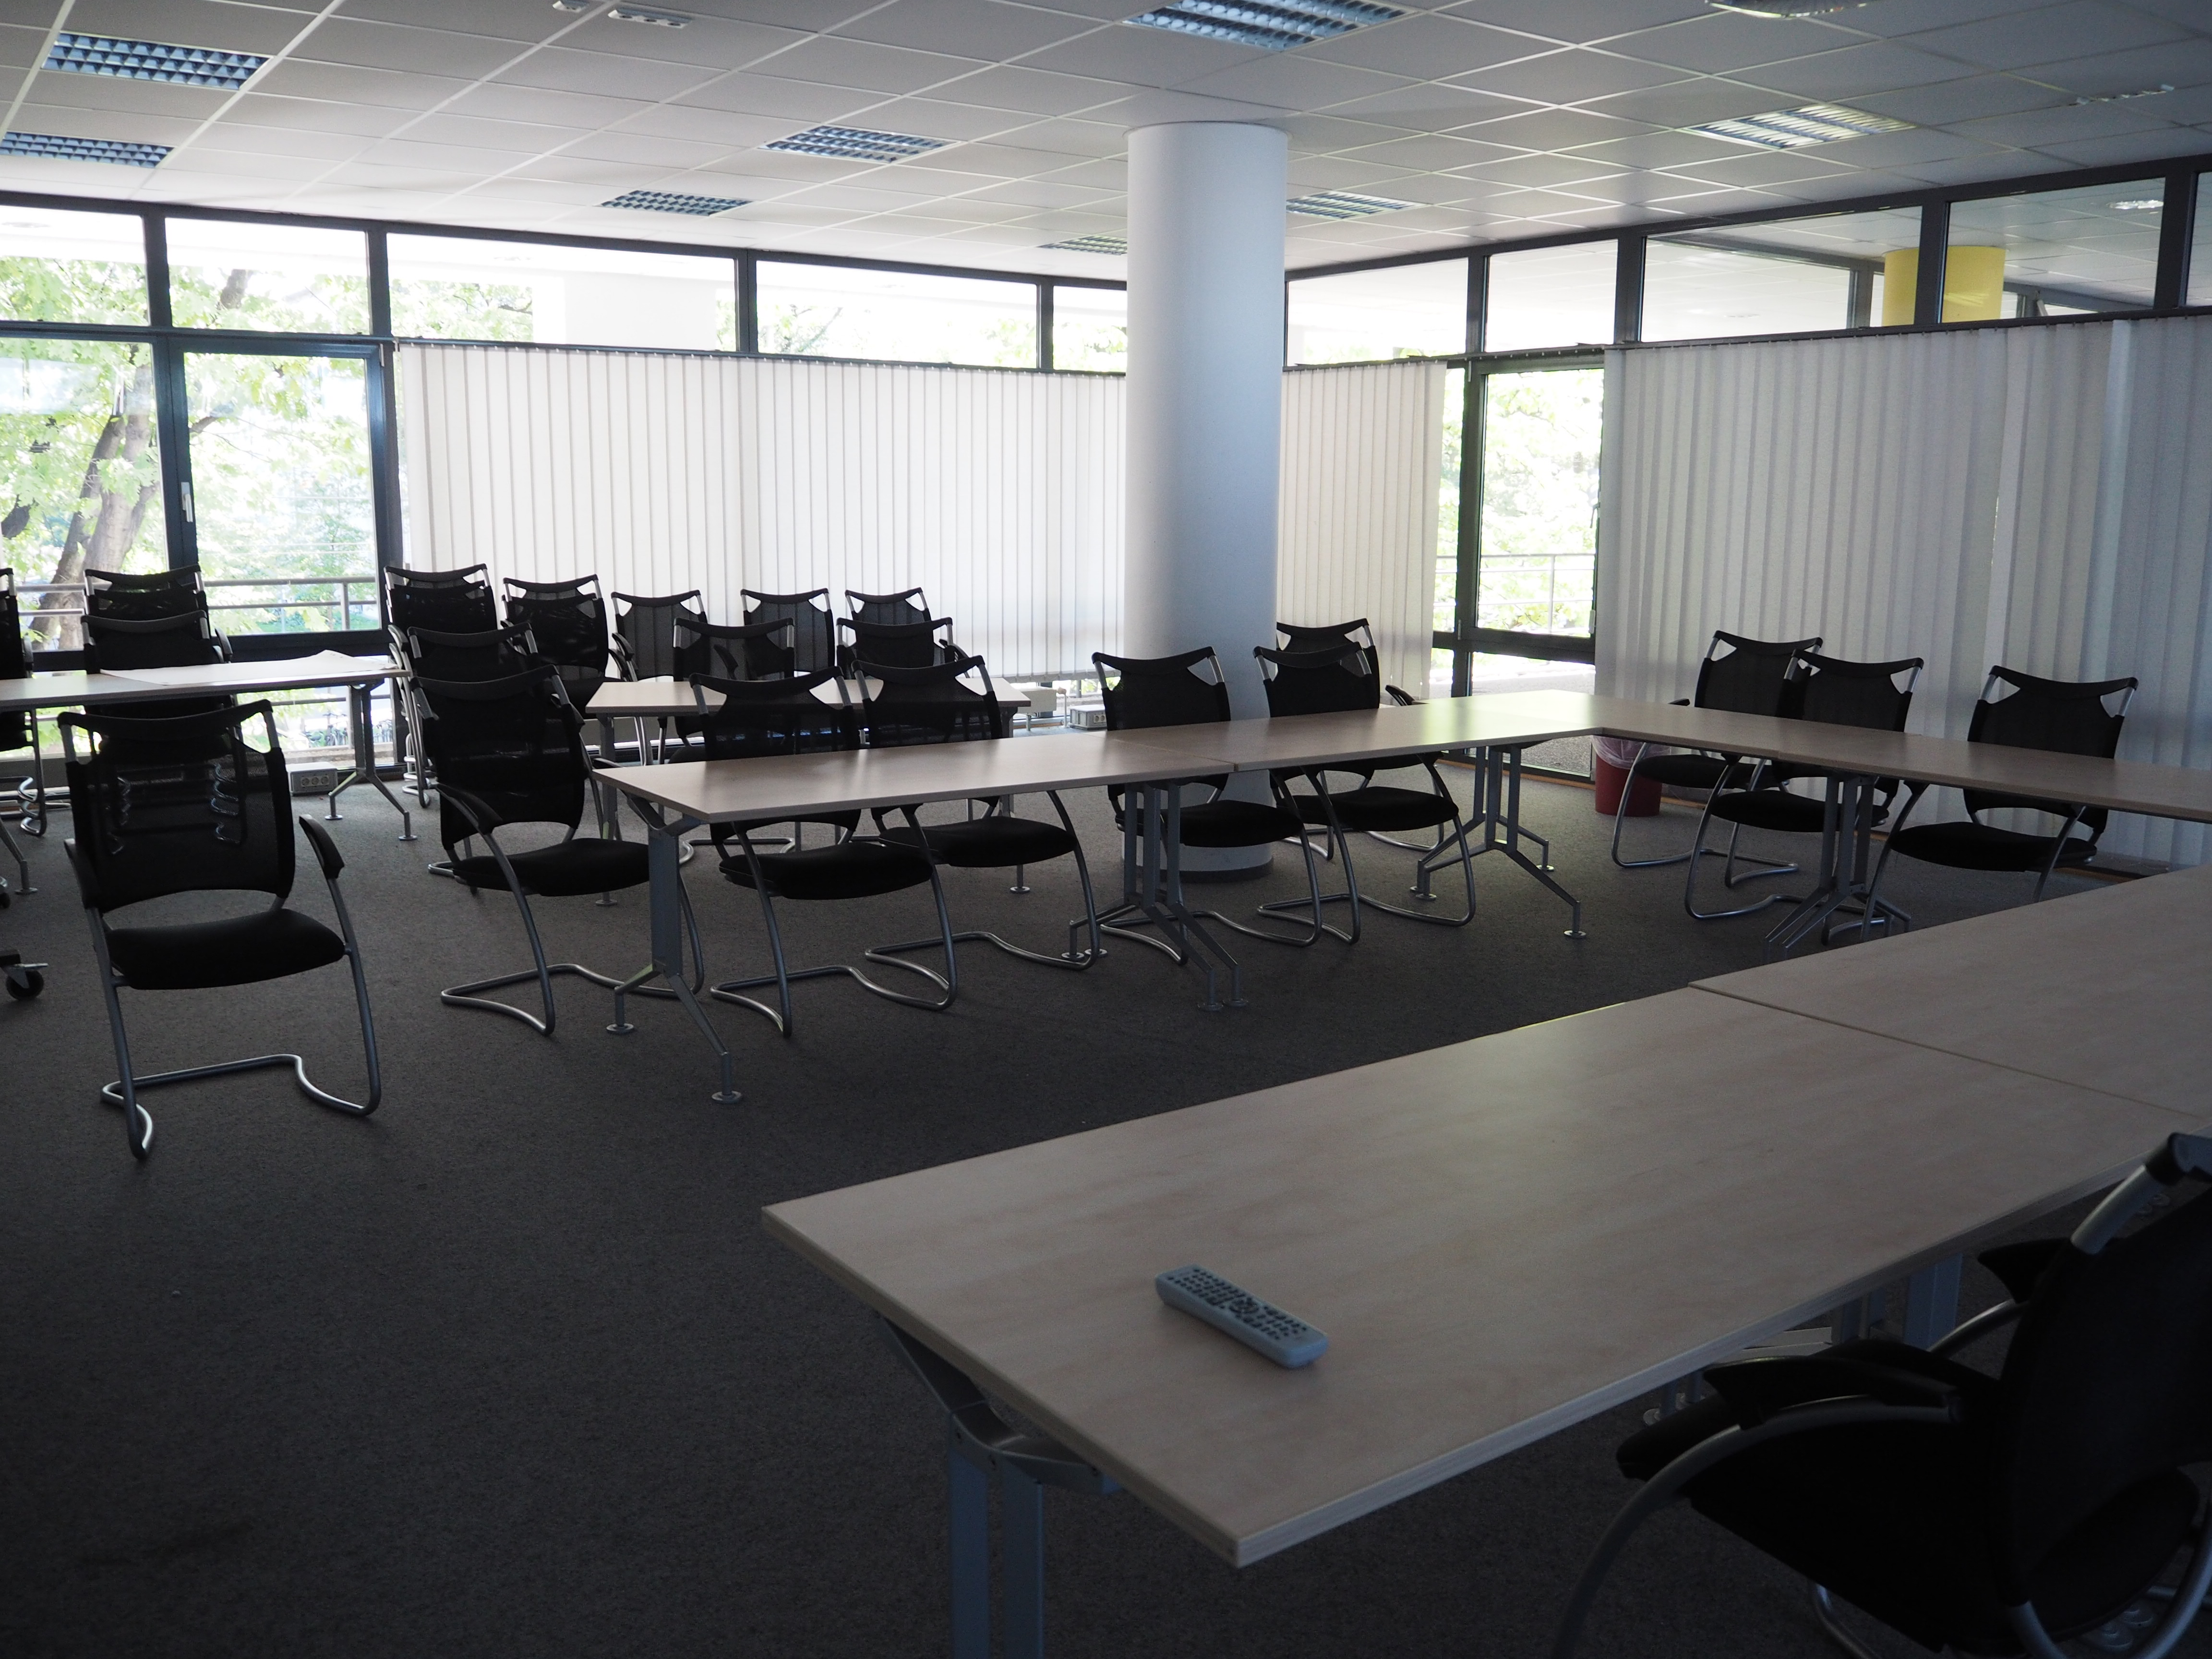
\includegraphics[width=0.25\linewidth]{images/venues/dhbw/P9280386}%
    };
  \end{scope}
  \node[anchor=south west,color=black,xshift=1ex,yshift=1ex] (label) at (sub-4.south west) {\imgtitle{Benjamin Berg}{Duale Hochschule Baden-Württemberg}{CC BY-SA 4.0}};
  \begin{scope}[on background layer]
    \node[fit=(label),inner sep=0,outer sep=0,opacity=0.6,fill=white,rounded corners] {};
  \end{scope}
\end{tikzpicture}


\begin{description}
\item[Location] off
\item[Price] gratis
\item[Rooms] audimax with 300 seats, many smaller ones
\item[Dates] end of July or later
\end{description}

The DHBW (Duale Hochschule Baden-Württemberg) offers exactly what we are looking for.
They have a large room for keynotes and some smaller rooms for talks and
also for BoFs in a single building. In addition to this the venue has
plenty of space in the lobby that we intend to transform into a lounge for
casual gatherings.

The venue is located further to the north west of the city, meaning that it is
unlikely to be within comfortable walking distance to the accommodation. However,
there is a tram station right next to the building and we are planning
to provide all attendees with tram tickets for the duration of the
conference. Furthermore if this location is chosen we are going to organize
lunch on-site as there are only limited options for lunch in the vicinity.

The venue is available from the end of July on.

\newpage

\begin{tikzpicture}[remember picture,overlay]
  \node[anchor=north west,outer sep=0,inner sep=0] (img) at (current page.north west) {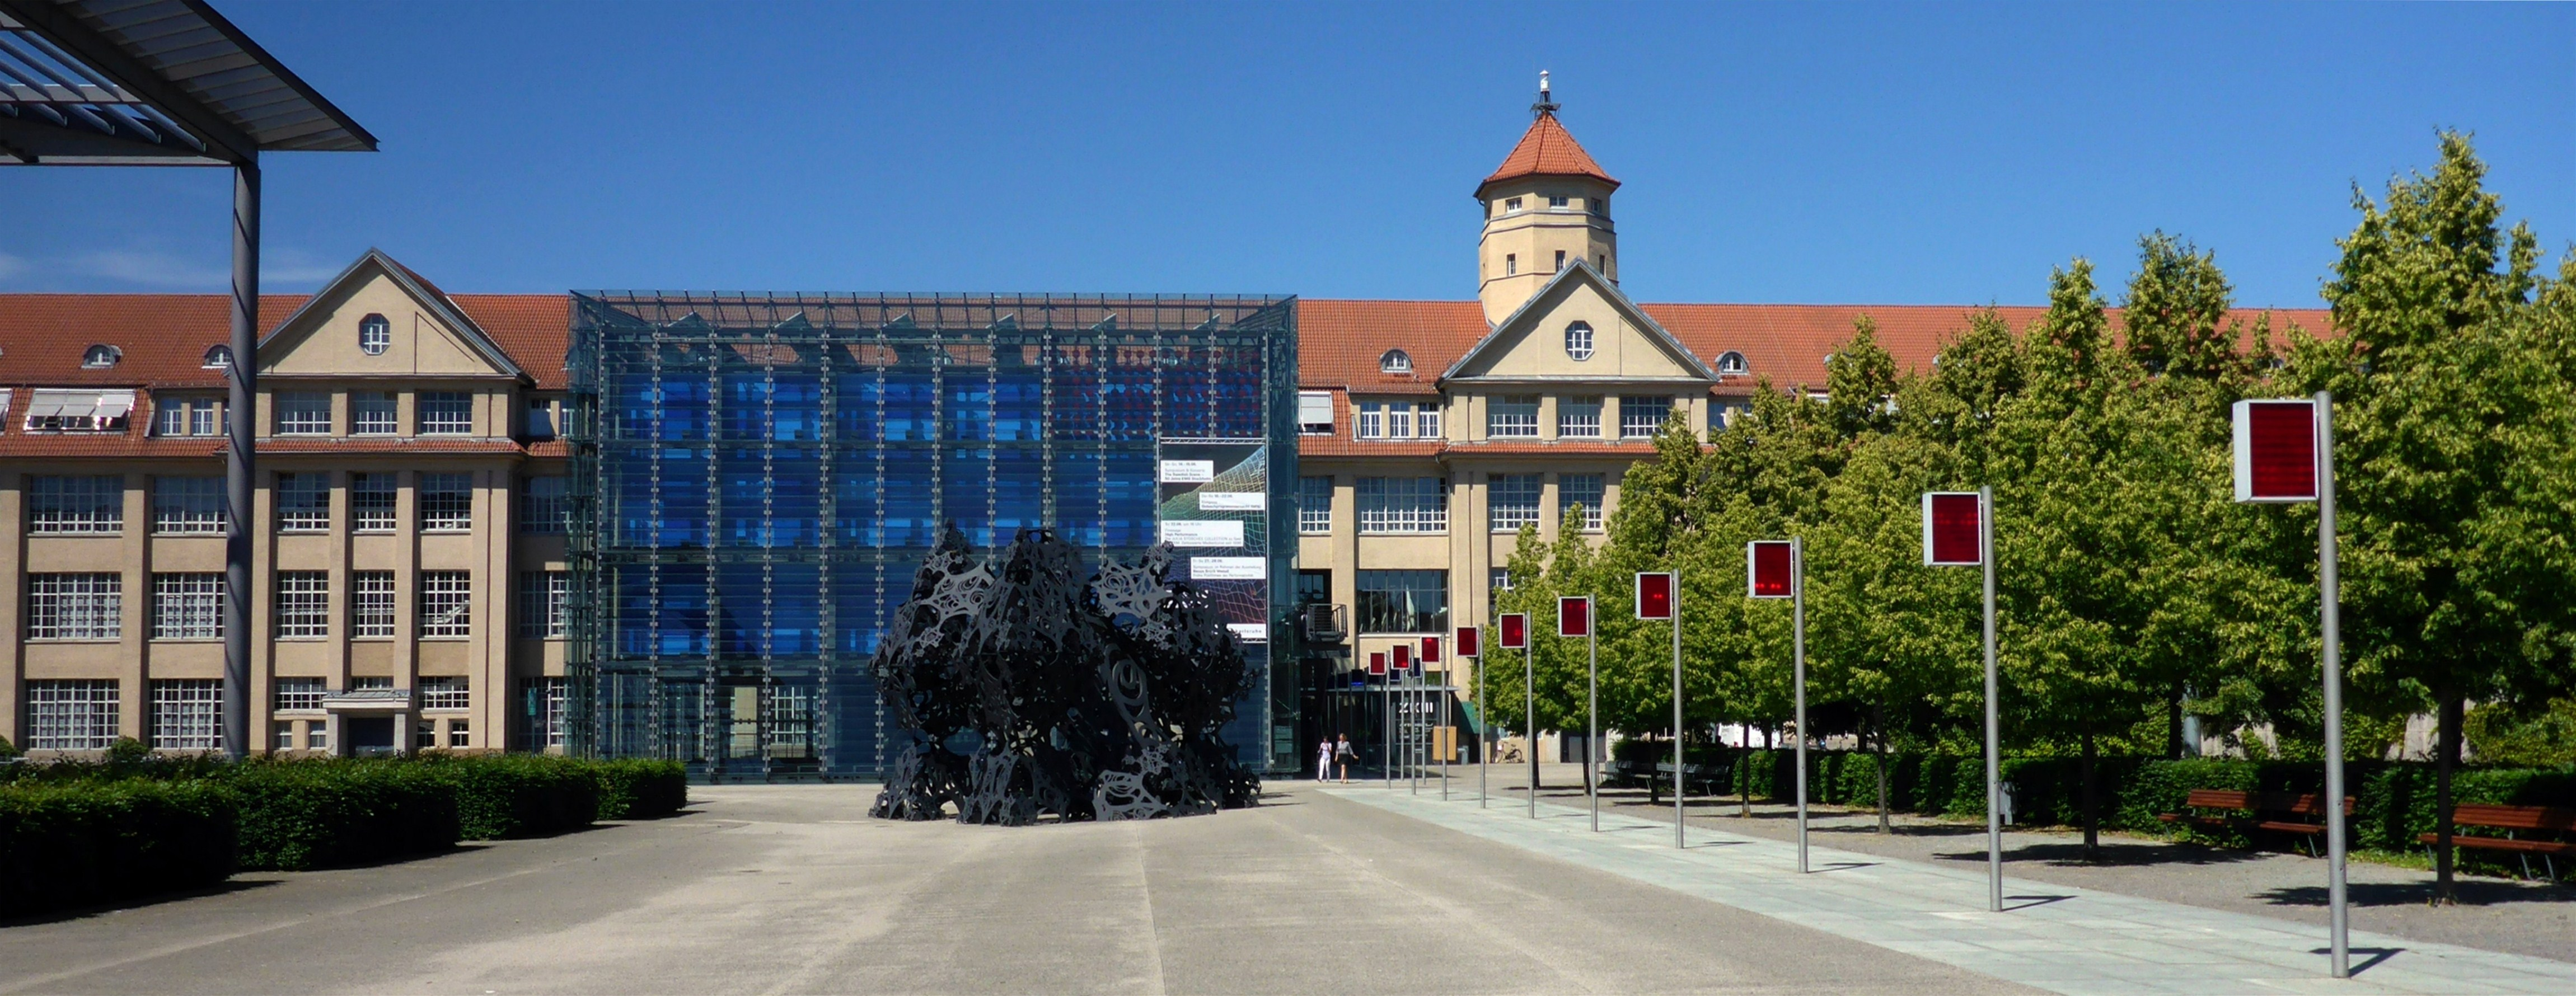
\includegraphics[width=21cm]{images/city/zkm-2.jpg}};
  \node[anchor=south west,outer sep=1ex,color=white] at (img.south west) {\imgtitle{Günter Josef Radig}{ZKM}{CC BY-NC-SA 2.0, not modified, \url{http://ka.stadtwiki.net/Datei:ZKM_2014.JPG}}};
\end{tikzpicture}

\vspace*{4.3cm}

\subsection{ZKM}
\begin{description}
\item[Location] very good
\item[Price] unknown, up to \SI{10000}{\euro}
\item[Rooms] one room with up to 300 seats, smaller auditorium with 100 seats
\item[Dates] 12.08.-14.08.\,2016
\end{description}

The Center for Art and Media (ZKM\footnote{Zentrum für Kunst und Medien}) is not
just a museum but a cultural institution that is unique throughout the world.
In the ZKMs own words, it is “a house for all media and genre, a house for both
spatially-based arts, such as painting, photography and sculpture as well as
time-based arts, such as film, video, media art, music, dance, theater, and performance.”

The venue has two auditoriums, the large “Medientheater” and a smaller
„Vortragsraum“. In addition to this there is a large lobby with a Café which we
would be sharing with the museum for the duration of the conference.

We would likely use this venue only for the core days, moving over to one of the
universities for the BoF sessions. As of now we have a reservation from the
12th to 14th of August but do not yet know the price we will be able to get.
For two core days this venue could cost up to \SI{10000}{\euro}.

\newpage


\begin{tikzpicture}[remember picture,overlay]
  \begin{scope}[on background layer]
    \node[anchor=north west,outer sep=0,inner sep=0] (img) at (current page.north west) {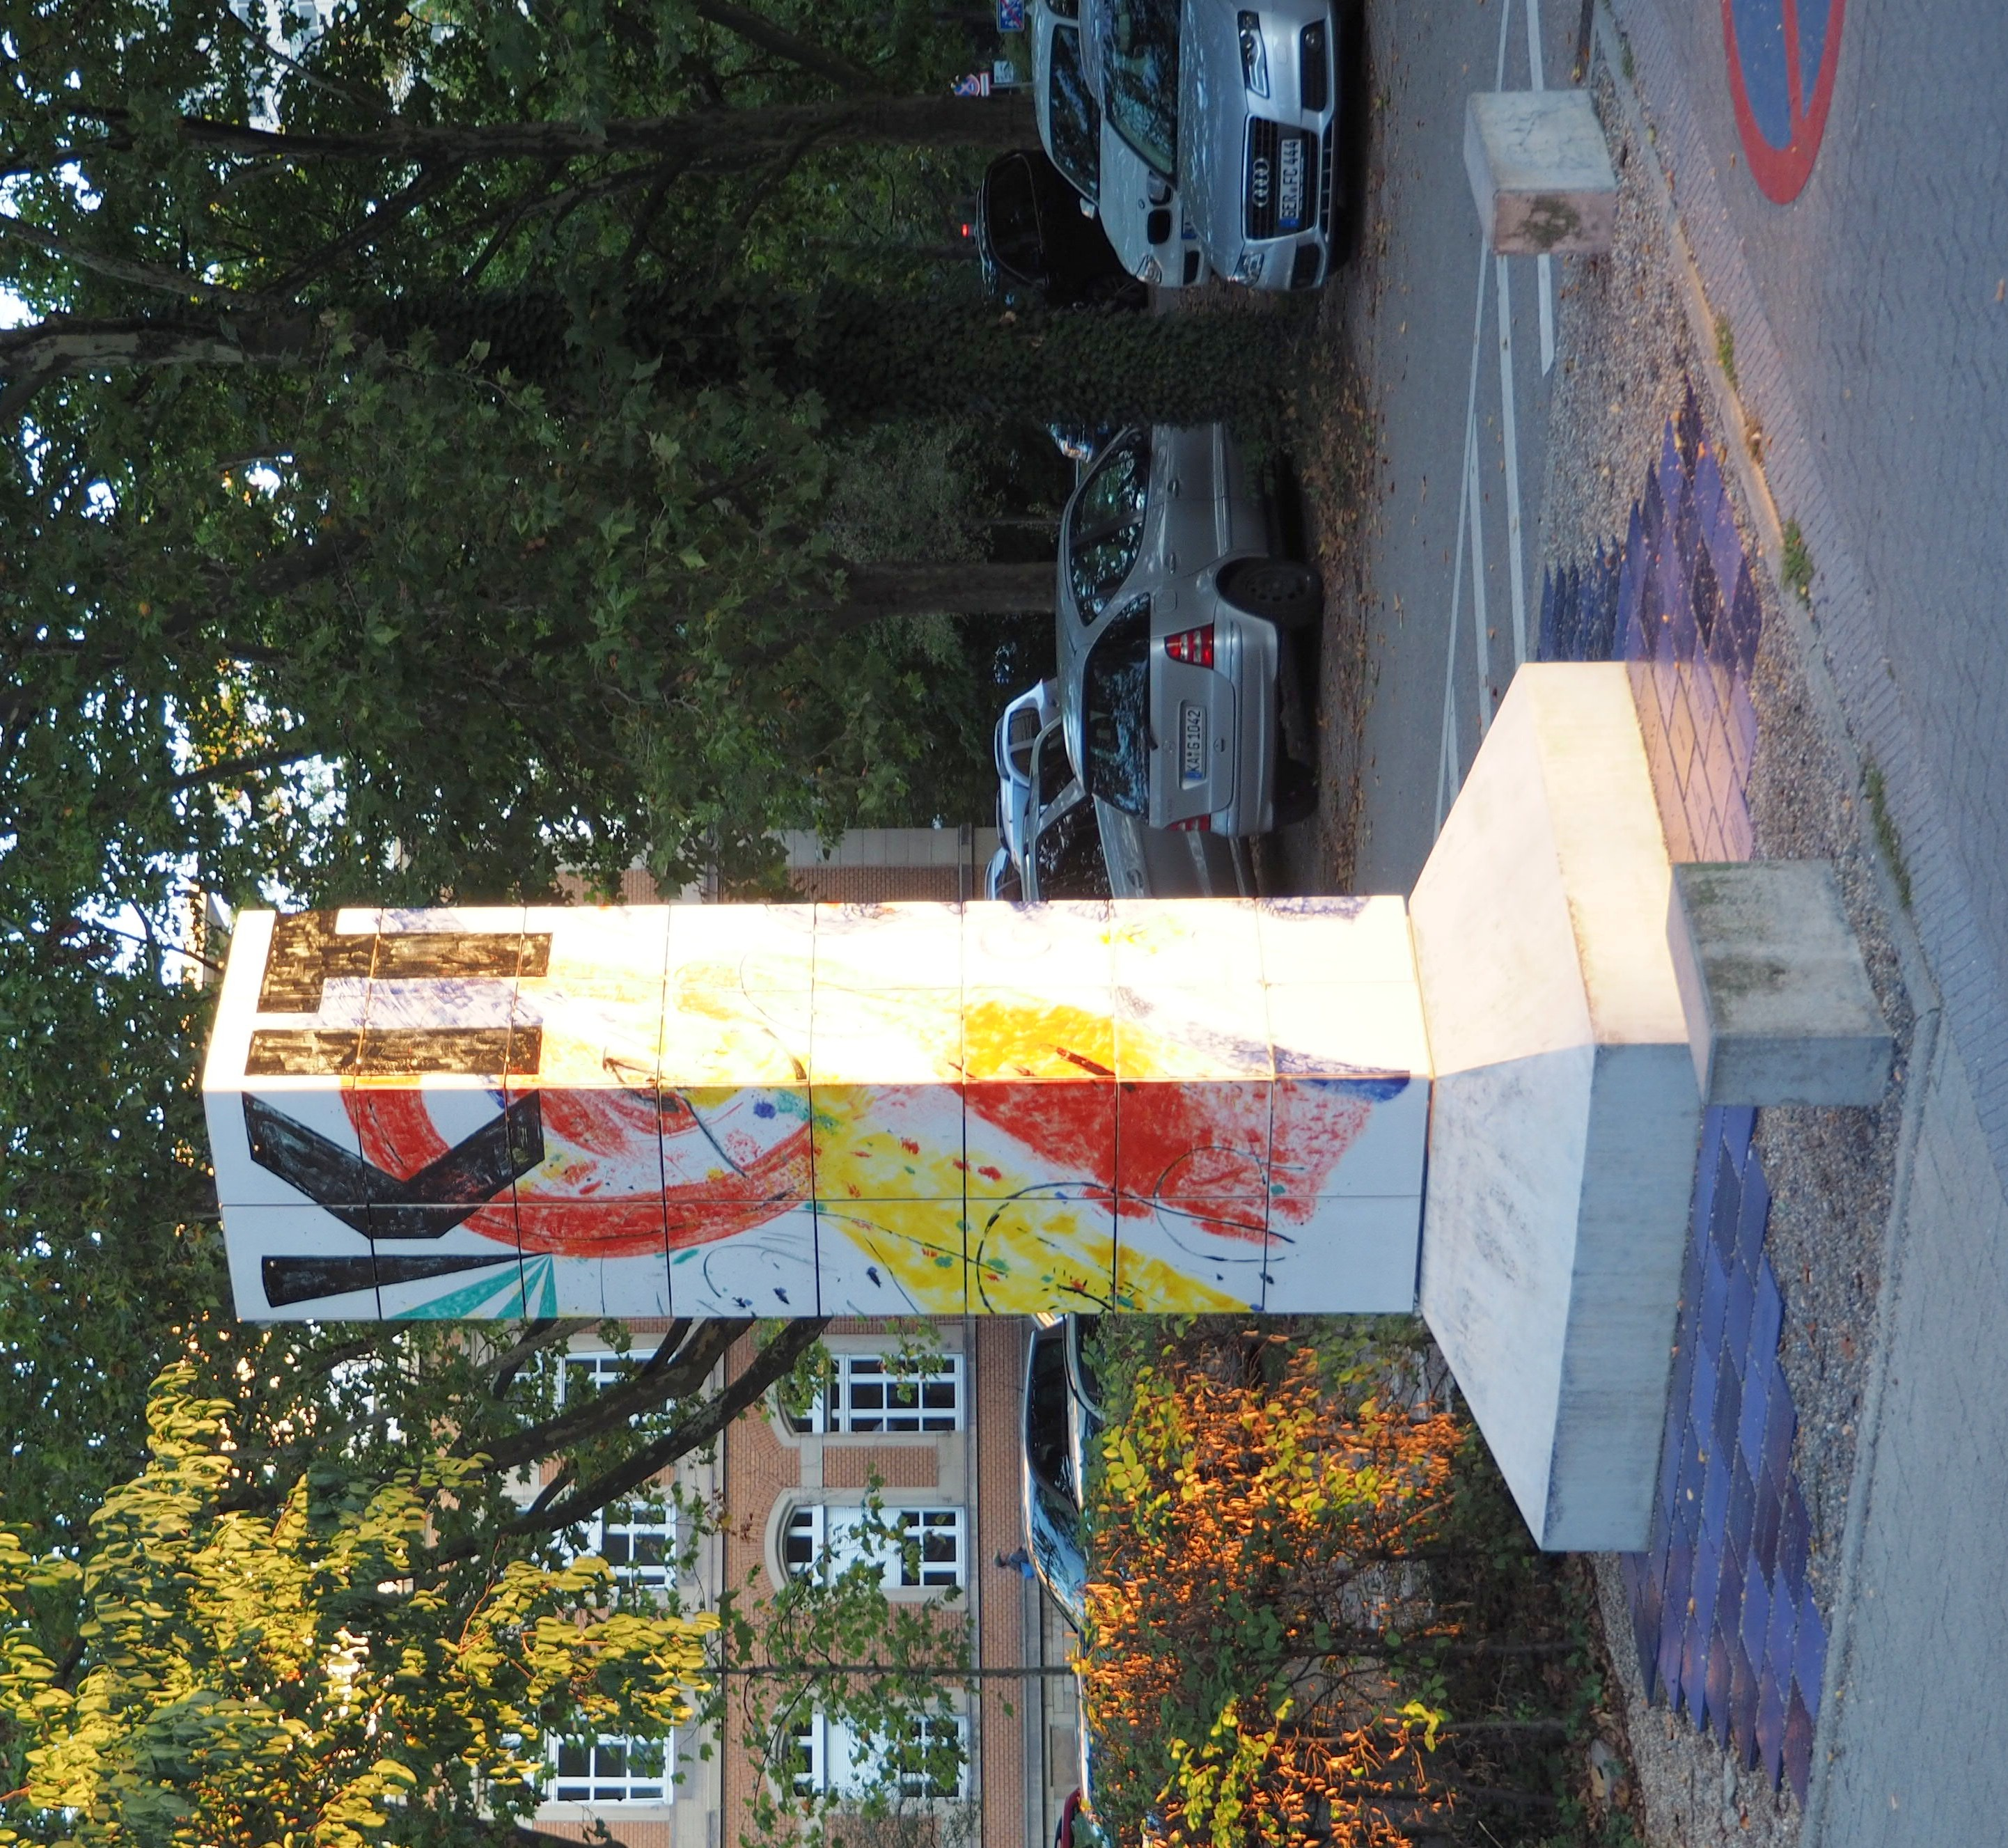
\includegraphics[width=9.5cm,angle=-90]{images/venues/kit/kit-1.jpg}};
    \node[anchor=north west,outer sep=0,inner sep=0,xshift=-1pt] (img-2) at (img.north east) {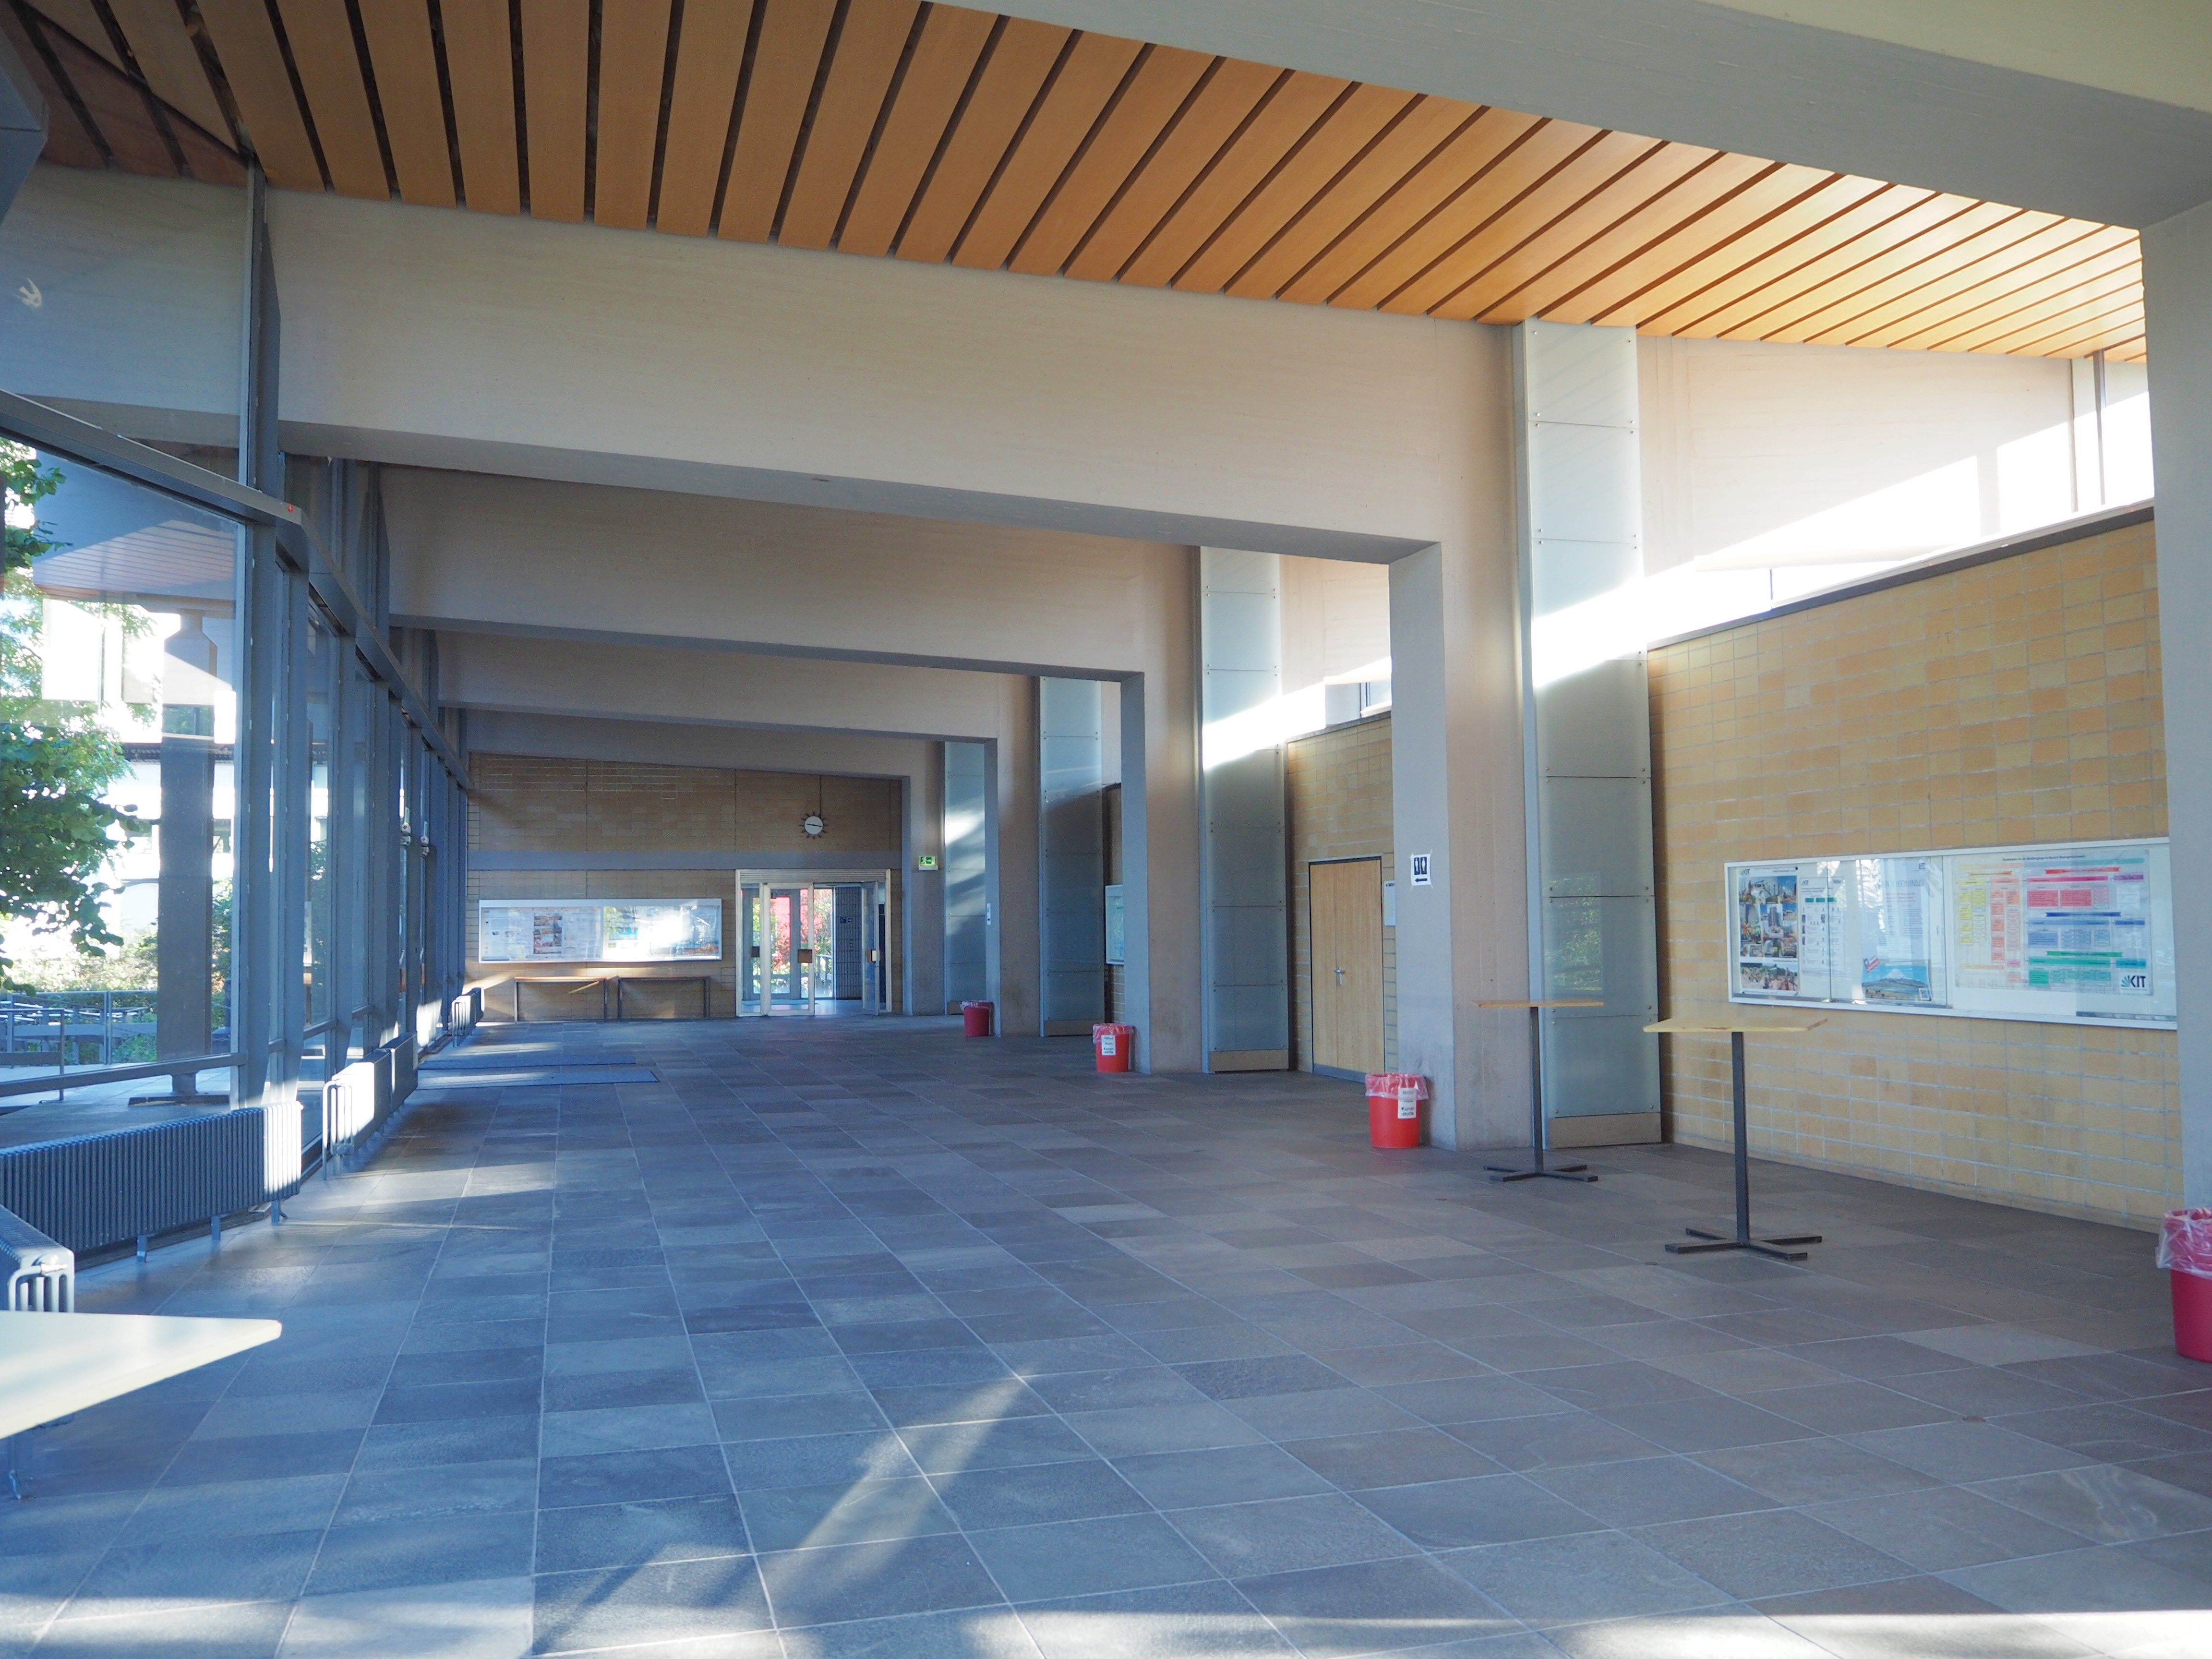
\includegraphics[height=9.5cm]{images/venues/kit/1050-1.jpg}};
  \end{scope}
  \node[anchor=south west,color=black,xshift=1ex,yshift=1ex] (label) at (img.south west) {\imgtitle{Benjamin Berg}{KIT and Building 10.50}{CC BY-SA 4.0}};
  \begin{scope}[on background layer]
    \node[fit=(label),inner sep=0,outer sep=0,opacity=0.6,fill=white,rounded corners] {};
  \end{scope}
\end{tikzpicture}

\vspace*{6cm}

\subsection{KIT south campus (University)}%\smash{\rlap{%
%\begin{tikzpicture}
%  \pgfsetbaselinepointlater{\pgfpointanchor{baseline}{base}}
%    \node[inner sep=0,outer sep=0] at (0pt,0pt) {};
%  \begin{scope}[on background layer]
%    \node[inner sep=0,outer sep=0,anchor=north east] (main) at (\linewidth,0em) {%
%      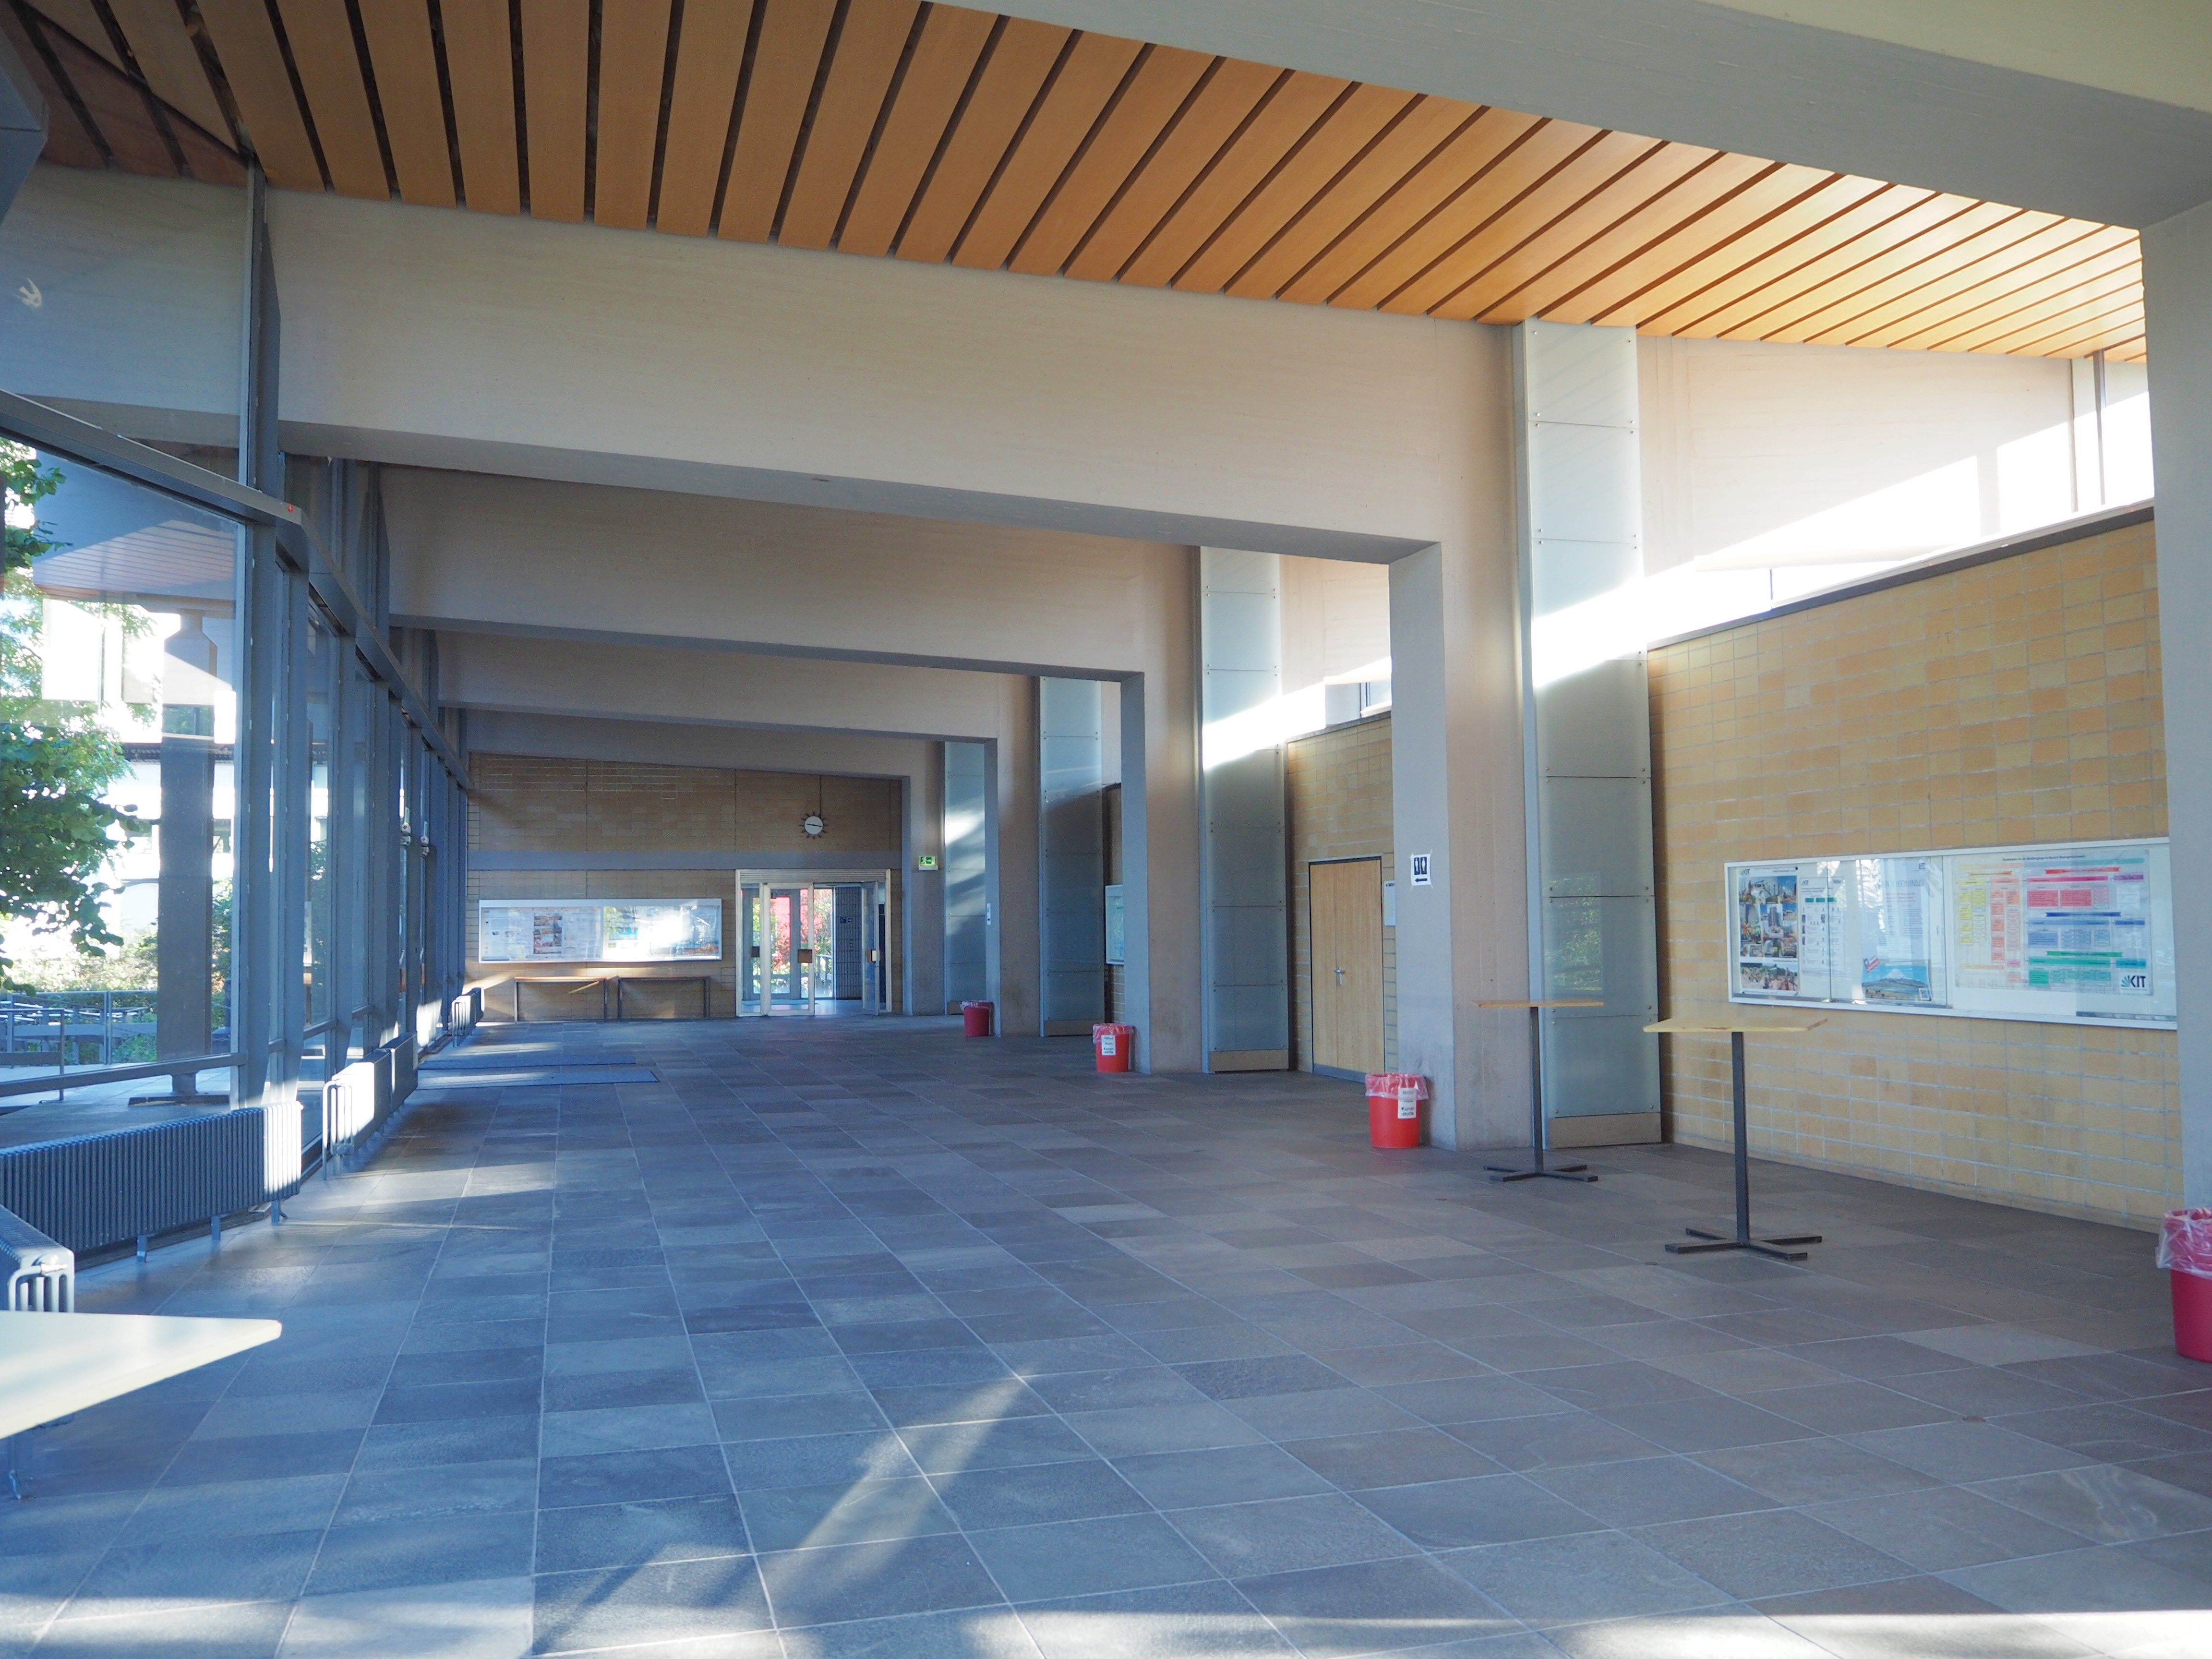
\includegraphics[width=0.4\linewidth]{images/venues/kit/1050-1.jpg}%
%    };
%    \node[coordinate] (baseline) at ($(main.north) + (0, -3em)$) {};
%  \end{scope}
%  \node[anchor=south west,color=black,xshift=1ex,yshift=1ex] (label) at (main.south west) {\rm\imgtitle{Benjamin Berg}{KIT Building 10.50}{CC BY-SA 4.0}};
%  \begin{scope}[on background layer]
%    \node[fit=(label),inner sep=0,outer sep=0,opacity=0.6,fill=white,rounded corners] {};
%  \end{scope}
%\end{tikzpicture}%
%%
%}}

\begin{description}
\item[Location] excellent
\item[Price] unknown
\item[Rooms] multiple possible locations
\item[Dates] earliest end of July, likely later
\end{description}

A third option is to hold the conference on the KIT south campus which is
located right next to the city center. Hosting the conference on the university
campus means that all social events and the city center would be within walking
distance from the venue.

Even though the computer science department is supporting the idea of holding
GUADEC at the KIT in Karlsruhe, we were not yet able to get a confirmation from
the KIT administration. We are in contact with the administration and the
information will be forwarded as soon as possible.

\subsection{Karlshochschule}
\begin{description}
\item[Location] very good
\item[Price] unknown
\item[Rooms] unknown
\end{description}

Another venue option we are currently in contact with is the centrally
located Karlshochschule. There is to be interested to host GUADEC which
might even happen in cooperation with the ZKM. However we were not yet able
to aquire more information as there were delays due to holidays and other reasons.

